% Chapter 1

\chapter{Starcraft II} % Main chapter title

\label{chap_sc2} % For referencing the chapter elsewhere, use \ref{Chapter1} 

%----------------------------------------------------------------------------------------
\section{Gameplay Basics}
Both Starcraft II and its Predecessor are Real Time Strategy(RTS) games set in the future. They are 2 of the most successful video games of their genre, with millions of players and active competitive scenes that award millions in tournament prizes each year. 

In StarCraft (II) the players take on the roles of the commanders of three different factions: Terrans, Zerg and Protoss.
While there is a single player campaign, the by far most played game mode is the competitive multi player 1 vs 1 ladder.
In this game mode the player starts with his races' main building and a group of workers.
His goal is to mine the 2 available resources Minerals and Gas with his workers and use these resources to build a base, by constructing different types of buildings and create an army using the unique unit types that are available to each race. While building and expanding his base and resource income the players use their units to attack their opponents' base or defend from their opponents' attacks. The game is over, when one player either gives up or has no more buildings on the map. This game mode is played on a number of different maps that offer distinct strategic possibilities through various base layouts, attack paths etc.

As a strategy game there are of course many different strategic choices to make.
These include when and how to build and expand your base, what unit composition to build your army with, when and where to attack and so on.
Much more than strategy, Starcraft II emphasizes the Real-Time aspect of RTS though. The main problem a Starcraft II player faces is how to to manage all the individual aspects of the game, like base building, managing the economy, scouting, micromanaging your army etc. simultaneously and as fast as possible. Even professional players, players that can often reach 300 Actions per Minute(APM) or more, can not multi-task efficiently enough to manage all these tasks perfectly. Such high APMs are achieved through the heavy use of hotkeys for unit and building groups, unit abilities and commands, and more.
In general, the game is controlled using Mouse and Keyboard, where the Keyboard is used mainly for around 30 different hotkeys and the mouse is used to move the screen around the map, select units or buildings and confirm orders needing a target mouse position.

In addition to multitasking another important challenge in Starcraft II is limited information. Due to a "Fog of War" that spans the entire map each player has only visibility in a small radius around each building and unit he owns. That means the players need to constantly scout the map and their opponent to get the information they need to make the correct Strategic choices.
There is also an inbuilt AI available in different difficulties that players can play against. This AI is hardcoded using traditional programming however and does not make use of machine learning. It is also very weak and should, even in the hardest difficulties that resort to cheating, prove almost no challenge to a decent Starcraft II player.

\begin{figure}[htb]
  \centering
      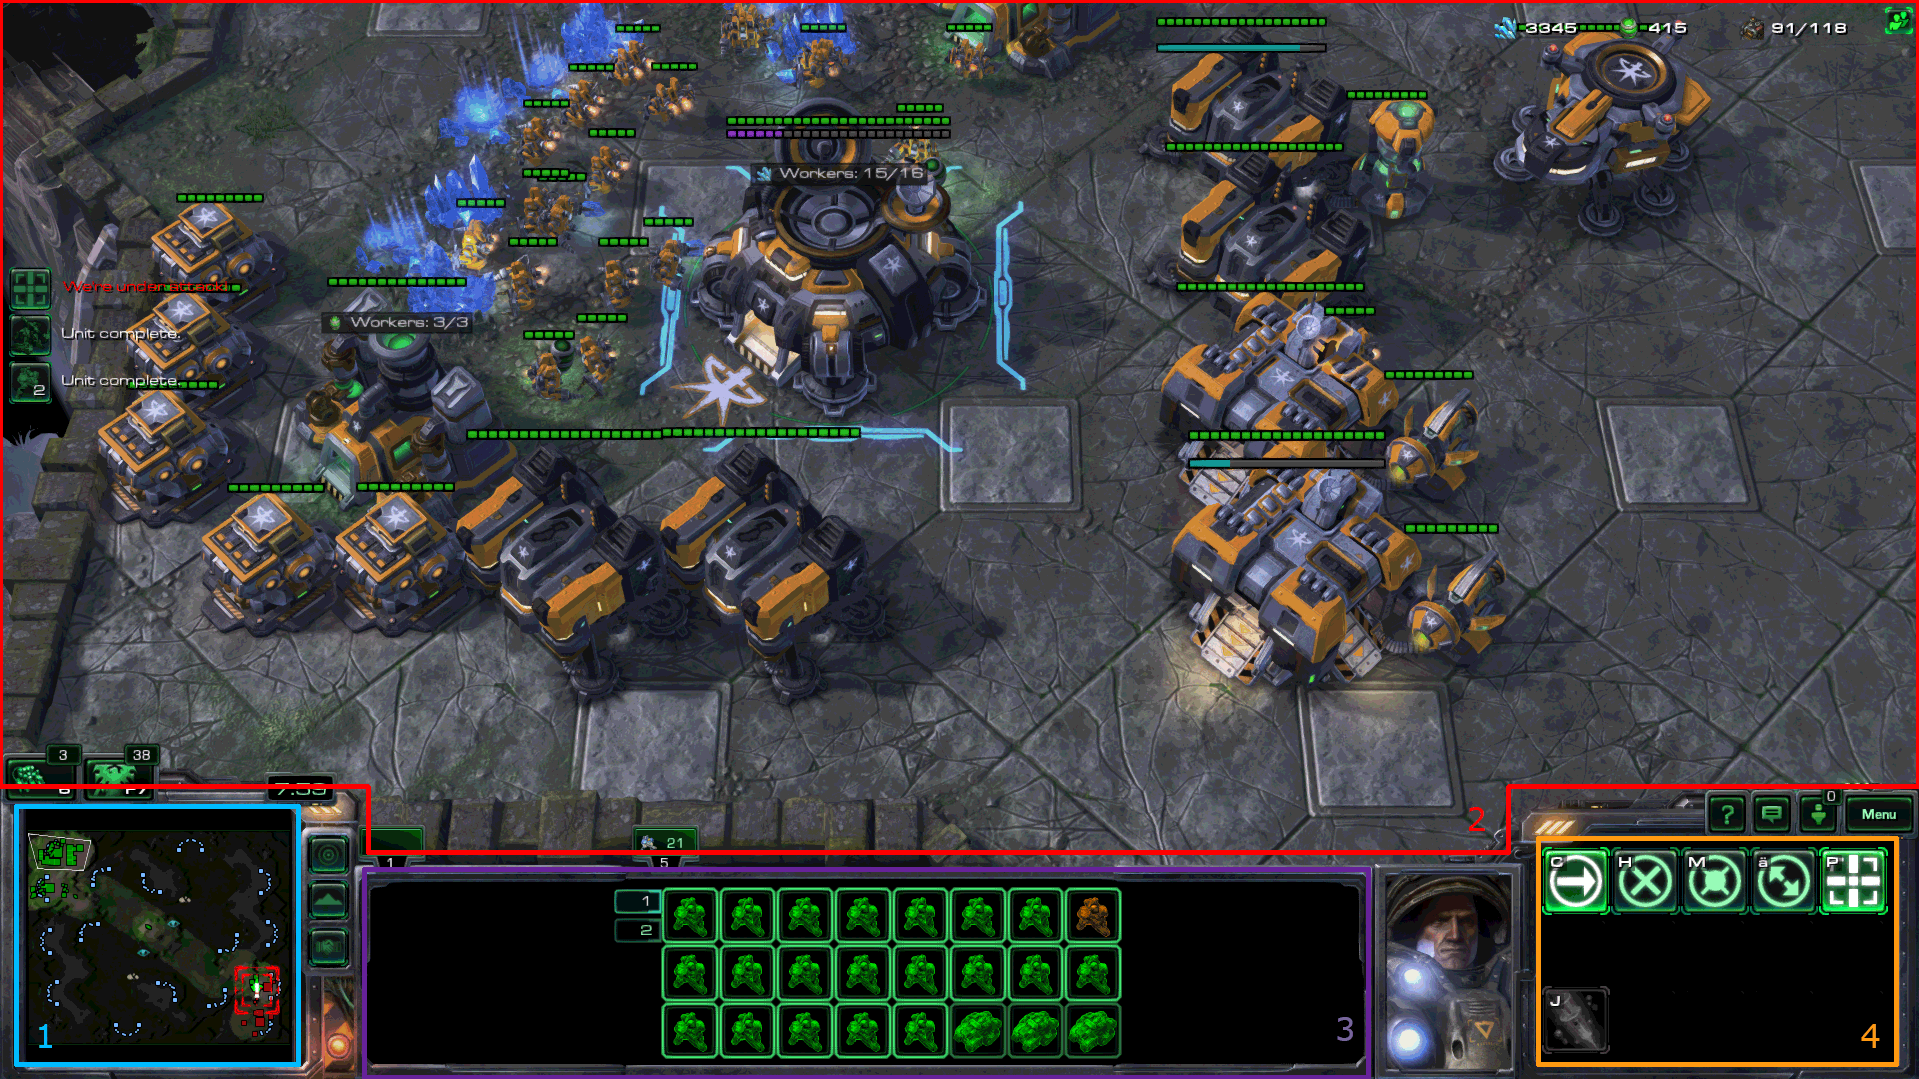
\includegraphics[width=1\textwidth]{Figures/gameview_bordered.png}
  \caption{The StarCraft II Ingame User Interface: 1 - Minimap view of the entire Map with white trapezoid showing current screen section, 2 - Main Game View, 3 - overview of currently selected unit(s), 4 - Command Palette of first unit type in selected units}
  \label{fig:gameview}
\end{figure}

Figure \ref{fig:gameview} show the default User Interface for a Terran player. The red bordered part of the screen is the main game view, that shows the actual game. Green bars over the units and denote their current hitpoints and change color depending on how much damage a unit has taken. Bordered in Teal is the minimap, which shows a minified view of the entire map with the white trapezoid being the section currently shown in the main game view. Friendly Units on the minimap are depicted in green, neutral units in yellow and enemy units in red. The purple section contains information about the currently selected units. Each square represents one unit and their color mirrors the color of their healthbar. The orange bordered section contains the command palette of the selected units or buildings, showing all actions that can be executed. Temporarily unavailable actions are greyed out. If multiple types of units are selected like in this screenshot, only the command palette for the first type of units is shown. That means that only their special abilities can be executed by a simple click or hotkey, using abilities of other unit types requires additional switching of the active unit type.


\section{Starcraft II as a Reinforcement Learning Environment}
The StarCraft games are well known as being very difficult to play both mechanically, meaning multitasking and just the general control of your mouse and keyboard, and strategically. The games have an incredibly high skill ceiling with even professional StarCraft players still making mistakes almost every game even after decades of competitive play and daily practise. The mechanical aspect of the game is where a computer should have a big advantage over human players as humans are physically limited in their APM. Strategy is something that one can expect an algorithm to struggle with much more, because it is a very creative and abstract aspect of the game. Both the mechanics and the strategy contribute to the high degree of  depth and complexity in the game. 

One tool that makes StarCraft II especially suited as a reinforcement learning environment is it's very powerful Map Editor. 
The StarCraft II Map Editor has played a big role in the success of Blizzard's Starcraft and also Warcraft video game franchises of Blizzard. It allows not only to create new maps for standard game modes, but gives so much freedom and access to game data and scripts, that it is very easy to create entirely new game modes that are entirely different. So much so, that sometimes the base game is barely recognizable anymore, because the game might not even be an RTS type game mode anymore. The most popular Genres of custom modes, also called "Fun Maps" or "UMS(Use Map Settings)"
 include Role Playing Games(RPGs), Co-Op shooters, Tower Defense, Survival, and many more.
 
Taking into account custom maps and game modes makes the number of possible scenarios that can be explored in StarCraft II using reinforcement learning almost infinite. Both this and the complexity of the game itself make for an, in my opinion, very interesting reinforcement learning environment. And, as demonstrated by the failure of the Deepmind Team to beat even the worst inbuilt AI using reinforcement learning \citep{DBLP:journals/corr/dmsc2}, it is an environment that will likely continue to present interesting challenges for AI Research in the foreseeable future.
 